\chapter{Fluid-Structure Interaction Problem Formulation}
The following chapter will be devoted to introducing the full FSI problem mathematically. The equations and interface conditions will be introduced in a strong and weak form. From the weak form both equations will be discretized into a scheme which will be used in the FSI solver. \newline

In describing the FSI problems the domain is split into three: fluid, structure, and interface. Fluid and structure domains are separated, and different constitutive equations are solved in each domain. The spatial points in which fluid and structure join is called the interface. The treatment of the interface separates the two most commonly used methods for solving FSI problems \cite{Liu2014}. The first method is called fully Eulerian. In a fully Eulerian framework, both the fluid and structure equations are defined and solved in a purely Eulerian description. The interface in a fully Eulerian framework is tracked across a fixed domain \cite{Valkov2015},which is a difficult task. The fully Eulerian description is suited for fluid problems but is problematic for structure problems because of the interface tracking. \newline

The second approach is the \textit{Arbitrary Lagrangian Eulerian} (ALE).
The ALE method entails formulating the fluid equations in a type of Eulerian framework and the solid in a Lagrangian framework. The entire domain itself moves with the structural displacements and the fluid moves through these points. In the ALE framework we get the best of both worlds, in that fluid and solid are described in their most commonly stated mathematical forms. The structure equation will remain as previously stated \eqref{eq:Solid}, and in the fluid equation we need to take into account the change in convection arising from the mesh deformation. \newline

Dealing with the movement of the domain is performed in two ways. One way is to move the domain itself in relation to the structural displacements, and use this new domain to calculate the equations for every iteration. This requires a specific function to move the mesh between each timestep. This process can be time consuming as problems get large. The structural deformation history can also give rise to problems as the points on the domain have changed location. \newline

The second approach to ALE, which will be used in this thesis, is to calculate from \textbf{reference domain}.
When solving equations from a reference frame we solve the equations on an initial, stress free domain, and use a series of mappings to account for the movements of the current time domain. It is the displacements in the domain that determines the value of the mappings between frames of reference. The solid equation is already stated in a Lagrangian formulation and does not need any mappings. It is the fluid velocities and fluid pressure that needs to be mapped from the reference domain into the time domain in which they are stated.
Since the reference frame method does not need a function to move the mesh between each time iteration, it can be less time consuming. The interface is also located in the same position, making the interface easy to track. With the domain always remaining the same variational coupling of forces is easier when computing from a reference domain.\newline

There are generally two different approaches when discretizing an FSI scheme. The first is a partitioned approach where fluid and structure are solved sequentially. The partitioned approach is appealing in that we have a wealth of knowledge and legacy code that can be used to solve each of these kinds of problems in an efficient manner. The difficulty however is dealing with the interface. There are kinematic and dynamic conditions that has to be fulfilled in FSI, and the coupling of these conditions is where problems arise. Artificial added mass can appear when a partitioned approach is used, arising from poorly coupling between fluid and solid velocities (This is discussed further in discussion chapter). However, in this thesis the monolithic approach is used. In the monolithic approach all of the equations are solved simultaneously. The monolithic approach has the advantage of offering numerical stability for problems with strong added-mass effects \cite{Liu2014}, and are fully coupled. The disadvantage over the partitioned approach is that we loose flexibility when solving many equations simultaneously, and the computing matrices can quickly become large, hence computationally costly and needing large memory. The overall ease of implementation and numerical stability makes monolithic the preferred choice in this thesis. \newline

The following chapter starts by introducing the mappings needed to change between current and reference domain. Lastly, the equations will be discretized following the notation and ideas from \cite{Richter2010}.

\section{Mapping Between Different Frames of Reference}
Figure \ref{pic:FSI_mapping} depicts a simple Fluid-Structure Interaction domain. The fluid is surrounded by elastic walls, like for instance a blood vessel. 
$\hat{\mathcal{S}}$ and $\hat{\mathcal{F}}$ denotes the solid and fluid reference domain respectively. $\hat{\Sigma}$ denotes the interface in the reference domain. $\partial\hat{\mathcal{F}}_{in}$ and $\partial\hat{\mathcal{F}}_{out}$ denotes the fluid in and outflow. $\partial \hat{\mathcal{S}}$ is the outer solid wall. The reference domain is mapped using $\chi^s$ and $\chi^f$ to the time domain denoted as $\mathcal{S}$ and $\mathcal{F}$. While the interface in the time domain is denoted as $\Sigma$

\begin{figure}[H]
\label{pic:FSI_mapping}
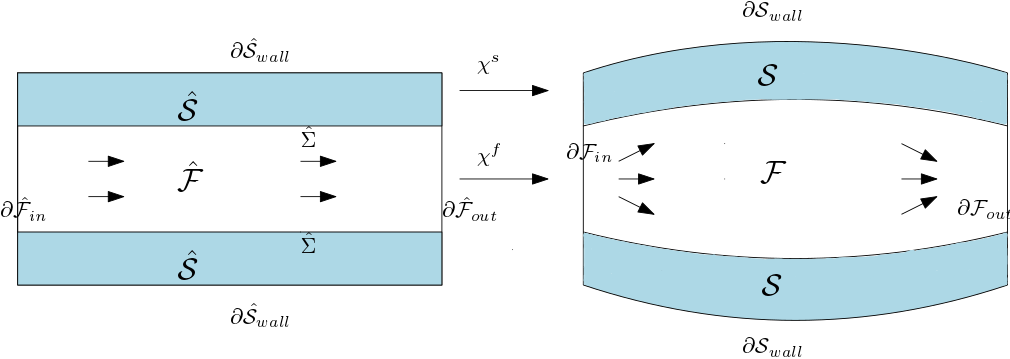
\includegraphics[scale=0.45]{./FSI_ALE_formulation/FSI_mapping.png}
\caption{Illustration of domain mapping}
\end{figure}

Let $\hat{\mathcal{V}}$ be a reference domain and $\mathcal{V}(t)$ be the current time domain. Then using the deformation gradient \eqref{eq:deformation_gradient} and the determinant of the deformation gradient named the Jacobian \eqref{eq:J}, to define a mapping between the volumes from the current to the reference configurations.

The Jacobian is used to map the domain from the current to the reference domain shown in equation \ref{eq:mappings1}, and the gradients acting on a vector $ \bold{u} $ will be mapped with the deformation gradient, shown in equation \ref{eq:mappings2}. Lastly the divergence of a vector $ \bold{u}$ will be mapped in a slightly different manner, shown in equation \ref{eq:mappings3}.

\begin{align}
\int_{\mathcal{V}(t)} 1  dx =& \int_{\hat{\mathcal{V}}} J dx  \label{eq:mappings1}\\
\int_{\mathcal{V}(t)} \nabla \bold{u}   dx =& \int_{\hat{\mathcal{V}}} J  \nabla \bold{u}F^{-1} dx \label{eq:mappings2} \\
\int_{\mathcal{V}(t)} \nabla \cdot \bold{u}   dx =& \int_{\hat{\mathcal{V}}} \nabla \cdot( J  F^{-1} \bold{u}) dx  \label{eq:mappings3}
\end{align}

\section{Governing Equations for Fluid-Structure Interaction}

The following section formulates the fluid and solid equations in the ALE description. The solid equation will remain in its Lagrangian description but the fluid equations will be changed in terms of the convective term and mapping between configurations. The derivatives in the different configurations are shown in \ref{deriv1}-\ref{eq:ALE}, to understand the need to change the the convective term in the fluid equation when stated in an ALE description \cite{Wick2011}:

\subsection{Derivatives in Different Frameworks}

In the Lagrangian framework the total and partial derivatives have the following relation:

\begin{equation}
D_t f(x,t) = \partial_t f(x,t) 
\label{deriv1}
\end{equation}

The total and partial derivatives have the following relation in the Eulerian framework, where $\bold{u}$ is the convecting velocity:

\begin{equation}
D_t f(x,t) = \bold{u}\cdot \nabla{f} + \partial_t f(x,t)
\label{deriv2}
\end{equation}

whilst in the ALE framework this concept is extended to take into account the motion of the domain:

\begin{equation}\label{eq:ALE}
D_t f(x,t) = \bold{w} \cdot\nabla{f} + \partial_t f(x,t)
\end{equation}

Equation \ref{eq:ALE} shows that in the Lagrangian framework $ \bold{w}$ is zero and for the Eulerian framework $\bold{w} = \bold{u}$.

\subsection{Solid Equation}
Let $\Omega \in \hat{\mathcal{S}} \cup \hat{\mathcal{F}} $ be a global domain that consists of the fluid, structure, and the interface. The interface is defined as: $ \hat{\Sigma} \in \hat{\mathcal{S}} \cap \hat{\mathcal{F}}  $. Let $\bold{u}$ be a global velocity function that describes the fluid velocity in the fluid domain and the structure velocity in the structure domain, $\bold{u} = \bold{u_s} \cup \bold{u_f} \in \Omega$. The deformation function is also defined as a global function $\bold{d} = \bold{d_s} \cup \bold{d_f} \in \Omega$. Using global velocity and displacement functions adds the feature of the velocity and displacement being continuous across the entire domain. This is an important feature which will be apparent once the interface conditions are stated. \newline 

The solid equation will be written in terms of the solid velocity $\bold{u_s}$, in contrast to \ref{eq:Solid} which was defined w.r.t the deformation $\bold{d}$. Defining the solid equation w.r.t to the deformation $\bold{d}$ can de done since the velocity is defined as the partial derivative of the deformation: $\bold{u} = \frac{\partial \bold{d}}{\partial t}$
The solid equation takes the following form in the Lagrangian formulation:
\begin{equation} \label{eq:solid}
\rho_s \frac{\partial \bold{u}}{\partial t} = \nabla \cdot (P) + \rho_s f \hspace{4mm}in\hspace{4mm} \hat{\mathcal{S}} 
\end{equation}

\subsection{Fluid Equations}
In the ALE description the fluid domain is moving, giving the need to redefine the velocity in the convective term in \eqref{eq:NS} to account for the moving domain: 
\begin{equation}
\bold{u} \cdot \nabla \bold{u} \rightarrow (\bold{u}-\frac{\partial \bold{d}}{\partial t}) \cdot \nabla \bold{u}  
\end{equation}
Where $\bold{d}$ is the deformation in the fluid domain. The domain velocity $\bold{w} = \frac{\partial \bold{d}}{\partial t}$ is defined w.r.t deformation as the partial time derivative.

Applying the mappings from \eqref{eq:mappings1}-\eqref{eq:mappings3} and including the mesh velocity in the convecting velocity as shown in \eqref{eq:ALE}, we end up with the fluid equations mapped from the time domain to the reference domain. These are shown in \ref{map1}-\ref{map5}, split up into a transient part, convection part, incompressible part, and the stress part:

\begin{align}
\int_{\mathcal{V}(t)} \rho_f \frac{\partial \bold{u}}{\partial t}  & = \int_{\hat{\mathcal{V}}}  \rho_f J \frac{\partial \bold{u}}{\partial t} dx \label{map1} \\
\int_{\mathcal{V}(t)} \nabla \bold{u} (\bold{u}-\frac{\partial d}{\partial t}) dx  &= \int_{J \hat{\mathcal{V}}} (\nabla \bold{u})F^{-1}(\bold{u}-\frac{\partial d}{\partial t}) dx  \label{map2}\\
\int_{\mathcal{V}(t)} \nabla \cdot \bold{u} dx  &=\int_{\hat{\mathcal{V}}}  \nabla \cdot (J F^{-1} \bold{u}  ) dx \label{map3} \\
\int_{\mathcal{V}(t)} \nabla \cdot \sigma_f dx &= \int_{\hat{\mathcal{V}}} \nabla \cdot( J F^{-1} \hat{\sigma_f} )     dx \label{map4} \\
\hat{\sigma_f} &= -pI + \mu ( \nabla \bold{u} F^{-1} + F^{-T} \bold{u}^{T}  ) \label{map5}
\end{align}

Assembling all these terms together gives strong form the fluid equations from a reference frame:

\begin{align}
\label{eq:NS_mapped}
\rho_f J \big( \frac{\partial \bold{u}}{\partial t} dx + (\nabla \bold{u})F^{-1}(\bold{u}-\frac{\partial \bold{d}}{\partial t}) \big) &= \nabla \cdot( J F^{-1} \hat{\sigma_f} ) + J \rho_f f \\
\nabla \cdot (J F^{-1} \bold{u} ) &= 0
\end{align} 

\section{Interface Conditions at the Boundary}
The fluid`s forces on the walls causes deformation in the solid domain and vice versa. The interface is where the energies between solid and fluid are transferred and we therefore need conditions on the interface. \newline

The three interface conditions comes from simple physical properties and consist of \cite{Richter2010}:
\begin{itemize}
\item \textit{Kinematic condition}: $\bold{u}_f = \bold{u}_s  \hspace{2mm} on \hspace{2mm} \hat{\Sigma}$. The fluid and structure velocities are equal on the interface, meaning the fluid moves with the interface at all times. 
Since we use a global function for $\bold{u}$ in both fluid and structure domains, this condition is upheld.
The fluid and solid velocities are usually in different coordinate systems, the solid velocity is then not available in Eulerian coordinates. We instead link fluid velocity at the interface by using the fact that $\bold{u}_s = \frac{\partial \bold{d}}{\partial t}$. Setting $\bold{u}_f = \frac{\partial \bold{d}}{\partial t}$ at the interface.

\item \textit{Dynamic condition}: $  \sigma_f n_f = \sigma_s n_s \hspace{2mm} on  \hspace{2mm}\hat{\Sigma}   $. \\
	The dynamic interface condition relates to Newtons third law of action and reaction. The forces on the interface area, here written as the normal forces are balanced on the interface. The forces from the fluid are defined in the time domain and is therefore written in terms of the reference domain: 
	$$J\sigma_f F^{-T} n_f = P n_s \hspace{2mm} on  \hspace{2mm}\hat{\Sigma} $$
	The dynamic condition is a Neumann condition that belongs to both subproblems.
	
\item \textit{Geometrical condition}: The geometric condition implies that the fluid and structure domains should not overlap, but rather that elements connect so the functions needing to transfer force are continuos across the entire domain.
\end{itemize}

\section{Methods for Domain Representation and Mesh Quality Preservation} \label{sec:meshmotion}
The kinematic interface conditions states that the fluid moves with the solid, and therefore the fluid domain needs to move in accordance with the solid deformations. The deformations from the structure are extrapolated through the interface into the fluid domain using, what is known in the literature as lifting operators. The lifting operators redistributes the interior node locations to uphold the mesh quality in the fluid domain.
The choice of lifting operator is important for the overall FSI problem to be calculated \cite{Wick2011a}. When large deformations occur, we need a good lifting operator to uphold the integrity of the computing domain. A poor choice may cause the cells to overlap and singularities may occur. In the best case the numerical solution diverges, in the worst case the numerical solution will be wrong.
When extrapolating deformation from the solid to the fluid domain, the fluid domain itself acts as a structure, deforming according to the deformations from the structure domain.\newline

I will in this section present different lifting operators, that act differently on the computational domain. In \ref{sec:mesh_motion} the techniques will be tested and investigated.

\subsection{Harmonic Lifting Operator}
The harmonic lifting operator can be used for small to moderate deformations. The harmonic lifting operator is the Laplace equation, transporting the deformations from the solid into the fluid domain. A variable $\alpha_u > 0$,which can be constant or varied spatially, can be multiplied to the Laplace equation, to control the amount of lifting of deformations to the fluid domain.

\begin{align}
 - \alpha_u \nabla^2 \bold{d} =& 0\hspace{4mm} in \hspace{2mm} \hat{\mathcal{F}}\\
  \hspace{4mm} \bold{d} =& 0 \hspace{4mm } on \hspace{2mm }  \partial \hat{\mathcal{F}} / \hat{\Sigma} \\
  \bold{d}_f =& \bold{d}_s \hspace{4mm } on \hspace{2mm } \hat{\Sigma} 
\end{align}

When using the harmonic lifting operator the variable $\alpha_u$ is very important when calculating moderate deformations. For small deformations a constant can be used for $\alpha_u$. But for larger deformations we need to be a bit more clever. A good strategy for choosing $\alpha_u$ was proposed by Wick in \cite{Wick2011a}, and further discussed in \cite{Stein2003} and \cite{MM2016}. This alpha gets bigger when closer to the interface: 
\begin{equation}
\alpha_u = \frac{1}{x^q}
\end{equation}
where $x^q$ is the distance from the interface. If $q=0$ the laplacian i recovered. When the distance becomes larger, $\alpha_u$ gets smaller, and vice versa. 
Defining $\alpha_u$ in this manner is a smart choice since it upholds the cell structure closer to the interface where most of the cell distortion appears. 

\begin{comment}
\subsection{Linear elastic extension}
Since the fluid domain acts as structure we can use a linear elastic equation to lift the deformations from the solid into the fluid domain. The linear elastic equation is best known from computing solid problems \cite{Wick2011a}.  The model is as follows:

\begin{align}
-\nabla \cdot \sigma_{mesh} &= 0 \hspace{4mm} in \hspace{2mm} \hat{\mathcal{F}}\\
\hspace{4mm} d &= 0 \hspace{4mm } on \hspace{2mm }  \partial \hat{\mathcal{F}} / \hat{\Sigma} \\
\sigma_{mesh} &= \alpha_\lambda (tr\epsilon)I + 2\alpha_\mu \epsilon 
\end{align}
where $\epsilon = \frac{1}{2}(\nabla d + (\nabla d)^T)$. $\epsilon$ is the linearized version of the strain tensor \eqref{eq:StrainTensor}. The parameters $\alpha_\lambda$ and $\alpha_\mu$ are chosen to uphold domain quality. This is performed by computing the parameters $\alpha_\lambda$ and $\alpha_\mu$ from Youngs modulus and poisson ration. 

\end{comment}

\subsection{Biharmonic Lifting Operator} 
The biharmonic lifting operator provides more freedom than the harmonic in choosing boundary conditions and choice of parameter $\alpha_u > 0$ \cite{MM2016,Wick2011a}. This is because the biharmonic extension, extends the deformation such that it upholds the integrity of the cells even in large deformations. In its simplest form it is written as:

\begin{equation}
- \alpha_u \nabla^4 \bold{d} = 0 \hspace{4mm}  in \hspace{2mm} \hat{\mathcal{F}}\\
\end{equation}

The biharmonic extension is calculated using a mixed formulation where we introduce a new function $\omega$ (not to be confused with the domain velocity), the function is added to the system so that we solve for 4 functions ($\bold{u}, \bold{d}, p, \text{and } \omega$):
 
\begin{equation}
\omega = \alpha_u \nabla^2 \bold{d} \hspace{4mm} and \hspace{4mm} - \alpha_u \nabla^2 \omega = 0 \hspace{2mm}   in \hspace{2mm} \hat{\mathcal{F}}
\end{equation}
with the two types of boundary conditions. The first boundary conditions being:
\begin{align}
\bold{d} = \partial_n \bold{d} =& 0 \hspace{4mm} on \hspace{2mm} \partial \hat{\mathcal{F}} \hspace{2mm} \textbackslash \hspace{2mm} \hat{\Sigma}\\
\bold{d}_f =& \bold{d}_s \hspace{4mm } on \hspace{2mm } \hat{\Sigma} 
\end{align}

The second type of boundary condition imposes conditions on $\bold{d}$ and $\omega$, and are written in terms of single component functions $\bold{d}^{(1)},\bold{d}^{(2)}$ and $\omega^{(1)}, \omega^{(2)}$, in the x and y directions.	
\begin{align}
\bold{d}^{(1)} =& \partial_n \bold{d}^{(1)} = 0 , and \hspace{4mm}   \omega^{(1)} = \partial_n \omega^{(1)} = 0    \hspace{4mm} on \hspace{2mm} \partial \hat{\mathcal{F}}_{in,out} \\
\bold{d}^{(2)} =& \partial_n \bold{d}^{(2)} = 0 , and \hspace{4mm}   \omega^{(2)} = \partial_n \omega^{(2)} = 0    \hspace{4mm} on \hspace{2mm} \partial \hat{\mathcal{F}}_{walls} \\
\end{align}

Since the biharmonic extension is a fourth order PDE, it will have a higher computational cost \cite{Richter2010} than the harmonic or linear elastic. 

\section{Discretization of monolithic FSI equations}\label{Discretization}
After introducing all the equations and boundary conditions needed to solve a FSI problem. We are ready to discretize the equations into one monolithic scheme. The equations will be discretized and solved using finite difference and finite element methods. I will introduce a so called $\theta$-scheme which will make it easy to implement different schemes, by choosing a value for $\theta$.
I will briefly introduce the spaces needed to discretize, following the ideas and notations of \cite{Wick2011}:

\subsubsection{Spaces}
Let $ X \in \mathbb{R}^d , d \in\{ 1,2  \} $ be a time dependent domain we define:

\begin{equation}
\hat{V}_X := H^1(X), \hspace{6mm}  \hat{V}^1_X := H^1_0(X) 
\end{equation}

$ H^1 $ indicating a Hilbert space and

\begin{equation}
\hat{L}_X := L^2(X), \hspace{6mm} \hat{L}^0_X := L^2(X) / \mathbb{R}
\end{equation}

$L^2$ indicating a standard Lebesque space.

The trial and test spaces for the velocity variable in the fluid domain,

\begin{equation}
\hat{V}^0_{f,u} := \{ \hat{u} \in H^1_0(\mathcal{F}) : \hat{u}_f = \hat{u}_s \hspace{2mm} on \hspace{2mm} \hat{\Sigma}  \}
\end{equation}

and the same for the artificial displacement in the moving fluid domain:

\begin{equation}
\hat{V}^0_{f,d} := \{ \hat{d} \in H^1_0(\mathcal{F}) : \hat{d}_f = \hat{d}_s \hspace{2mm} on \hspace{2mm} \hat{\Sigma}  \}
\end{equation}
\begin{equation}
\hat{V}^0_{f,d} := \{ \hat{d} \in H^1_0(\mathcal{F}) : \hat{\psi_f} = \hat{\psi_s} \hspace{2mm} on \hspace{2mm} \hat{\Sigma}  \}
\end{equation}

Now that the spaces have been defined we are ready to discretize. The temporal discretization is done using finite difference schemes and the spatial is treated with the finite element method. I will employ a $\theta-$ scheme that will enables us to easily switch between schemes.

\subsubsection{Discretization}

In the domain $\Omega$ and time interval [0,T]:

Find $ U = \{\bold{u}, d, p\} \in \hat{X}^0_D $ where $ \hat{X}^0_D := \{ \bold{u}^D_f + \hat{V}^0_{f,\bold{u}} \} \times \hat{L}_f \times \{ d_f^D + \hat{V}^0_{f,\hat{f}} \} \times \{ d_f^D + \hat{V}^0_{f,\hat{f}} \} \times \hat{L}^0_f \times \hat{L}^0_s  $ such that:

\begin{equation}
\int_0^T A(U)(\Psi) dt = \int_0^T \hat{F}(\Psi) dt \hspace{4mm} \forall  \Psi \in \hat{X}
\end{equation}

where $ \Psi = \{\phi, \psi, \gamma \} $% \hat{\psi}^\bold{u}_f, \hat{\psi}^\bold{u}_s, \hat{\psi}^d_f, \hat{\psi}^d_s, \hat{\psi}^p_f,\hat{\psi}^p_f  \}$ and

 $\hat{X} = \hat{V}^0_{f,\bold{u}} \times \hat{L}_f \times \hat{V}^0_{f,d,\hat{\Sigma}} \times \hat{V}_s^0 \times \hat{L}_f^0 \times \hat{L}_s^0  $


I first introduce the scheme using, for simplicity, the harmonic mesh motion. Let $\bold{u}$ be a global function in the entire domain instead of $\bold{u}_f$ in the fluid and $\bold{u}_s$ in the solid. Same for the test functions. This is done for ease of reading and also for the ease of implementation later.

\textbf{The full monolithic FSI variational form reads}:
\begin{align}
A(U)&= (J \rho_f \partial_t \bold{u} , \phi ) - (J (\nabla u)F^{-1}(\bold{u} - \partial_t d) , \phi )_{\mathcal{\hat{F}}}  \\
       &+ ( J \sigma_{f} F^{-T} , \nabla \phi )_{\mathcal{\hat{F}}} \\
       &+ (\rho_s \partial_t \bold{u} , \phi)_{\mathcal{\hat{S}}}   + \big(F S_s, \nabla \phi \big)_{\mathcal{\hat{S}}} \\
       &+ ( \alpha_u \nabla \bold{u}, \nabla \psi)_{\mathcal{\hat{F}}} + (\nabla \cdot (J F^{-1} \bold{u}),\gamma )_{\mathcal{\hat{F}}} \\
       \label{eq:condition}
       &+ \delta\big((\partial_t \bold{d} , \psi)_{\mathcal{\hat{S}}}  - ( \bold{u} , \psi )_{\mathcal{\hat{S}}}\big) \\ 
       &+  \big( J \sigma_{f,p} F^{-T}, \nabla \phi  \big) 	 		
\end{align}

The condition \eqref{eq:condition} , is weighted with a $\delta$ value. This is a critical detail for the program (detailed later) to run. The only two places where we use the test function $\psi$ is on this condition and the lifting operator. The weighting says in a weak manner that this condition is important for the overall program. \newline

I will here formulate the \textit{One step-$\theta$ scheme} from \cite{Wick2011}. This $\theta$ scheme has the advantage of easily being changed from the backward (implicit), forward(excplicit) or Crank-Nicholson (implicit) scheme. The Crank-Nicholson scheme is of second order, but suffers from instabilities in this monolithic scheme \cite{Wick2011}. A remedy for these instabilities is to chose a Crank-Nicholson scheme that is shifted towards the implicit side. How this is done will become evident once the scheme is defined.

We define the variational form by dividing into four categories, this may seem strenuous at first but the need for it will become evident when implementing the $\theta$-scheme. The four divided categories consists of: a time term, implicit, pressure and the rest (stress, convection):

\begin{align}
A_T(U) &= (J \rho_f \partial_t \bold{u} , \phi ) - (J (\nabla u)F^{-1}(\partial_t \bold{d}) , \phi )_{\mathcal{\hat{F}}} \\
	    & + (\rho_s \partial_t \bold{u} , \phi)_{\mathcal{\hat{S}}} + (\partial_t \bold{d} , \psi)_{\mathcal{\hat{S}}}  \\
A_I(U) &= ( \alpha_u \nabla \bold{u}, \nabla \psi)_{\mathcal{\hat{F}}} + (\nabla \cdot (J F^{-1} \bold{u}), \gamma)_{\mathcal{\hat{F}}} \\
A_E(U) &= (J (\nabla u)F^{-1} \bold{u} , \phi )_{\mathcal{\hat{F}}} + ( J \sigma_{f,u} F^{-T} , \nabla \phi )_{\mathcal{\hat{F}}} \\
	    & + \big(F S_s, \nabla \phi \big)_{\mathcal{\hat{S}}} - ( \bold{u} , \psi )_{\mathcal{\hat{S}}} \\
A_P(U) &= \big( J \sigma_{f,p} F^{-T}, \nabla \phi  \big)  	 		
\end{align}

Notice that the stress tensors have been split into a velocity and pressure part. 
\begin{align}
\sigma_{f,u} &= \mu ( \nabla u F^{-1} + F^{-T} \nabla u) \\
\sigma_{f,p} &= -p I
\end{align}

For the time group, discretization is done in the following way:
\begin{align}
A_T(U^{n,k}) \approx & \frac{1}{k} \big( \rho_f J^{n,\theta} (\bold{u}^n - \bold{u}^{n-1}) , \phi  \big)_{\mathcal{\hat{F}}} - \frac{1}{k} \big( \rho_f (\nabla u ) (\bold{d}^n - \bold{d}^{n-1}) , \phi \big)_{\mathcal{\hat{F}}} \\
+ & \frac{1}{k} \big( \rho_s  (\bold{u}^n - \bold{u}^{n-1}) , \phi  \big)_{\mathcal{\hat{S}}} +  \frac{1}{k} \big( (\bold{d}^n - \bold{d}^{n-1}) , \psi  \big)_{\mathcal{\hat{S}}}
\end{align}
And the Jacobian is written with superscript $\theta$ as:

\begin{equation}
J^{n, \theta} = \theta J^n + (1-\theta)J^{n-1}
\end{equation}

We can now introduce the \textit{One step-$\theta$ scheme}: 
Find $U^n = \{\bold{u}^n , \bold{d}^n, p^n \}$

\begin{align}
& A_T(U^{n,k}) + \theta A_E(U^{n}) + A_P(U^{n}) + A_I(U^{n}) = \\
& - (1-\theta) A_E(U^{n-1}) + \theta \hat{f}^n + (1-\theta) \hat{f}^{n-1}  
\end{align}

We notice that the scheme is selected by the choice of $\theta $. By choosing $ \theta = 1$ we get the back Euler scheme, for $ \theta = \frac{1}{2}$ we get the Crank-Nicholson scheme and for the shifted Crank-Nicholson we set $ \theta = \frac{1}{2} + k$, effectively shifting the scheme towards the implicit side. $\hat{f}$ is the body forces which will be ignored in this thesis. The shifting toward the implicit side is important for long term stability for certain time step values \cite{Wick2011}. The shifting will be investigated in the next chapter.







\begin{comment}
\subsection{Spaces and Elements}
The velocity and pressure copling in the fluid domain must satisfy the inf-sup condition. If not stabilization has to added. We here need to define some spaces that will have these desired properties.
We denote $u_h \in V_h$ and $ d_h \in W_h $, here the finite element pair og pressure and velocity mush satisfy the inf-sup condition given in ALE coordinates:
$$   \inf_{\substack{p_h \in L_{h,f}}}  \sup_{\substack{v_h \in V_{h,f}}} \frac{ (p_h, div(J_f F_f^{-1} u_h))_{\mathcal{F}} }{ \|\|J^{\frac{1}{2}} p_h  \|\|_{\mathcal{F}} \|\|  J^{\frac{1}{2}}_{f} \nabla u_h F_f^{-T} \|\|_{\mathcal{F}}  } \geq \hat{\Sigma}     $$
A good choice of spaces will be P2-P2-P1 for velocity, displacement and fluid pressure respectively. 
\end{comment}







